\documentclass{article}
\usepackage[utf8]{inputenc}
%\usepackage{german}
\usepackage{color} %Zum stylen von \def
\usepackage{varwidth} %Zum stylen von \def
\usepackage{etoolbox} %Zum stylen von \def
\usepackage{amssymb} %Für die Mengensymbole
%\usepackage{svg}
\usepackage{graphicx}
\graphicspath{ {./images/} }
\usepackage{amsmath} %Zur Darstellung von Funktionen mit Fallunterscheidung
\usepackage{scrlayer-scrpage} %Kopf- und Fusszeile
\usepackage{titling} %Titel nach oben verschieben
\usepackage{amsfonts} %\mathcal
\usepackage{enumerate} %Für kleine römische Zahlen in Aufzählungen


%\usepackage{prettyref}
%\usepackage{apacite}
\usepackage[
backend=biber,
style=apa,
]{biblatex}
\addbibresource{references.bib}

%\usepackage{array,multirow}



%% Formatierung %%
\usepackage[dvipdfm]{geometry}
\setlength{\droptitle}{-10em}
\geometry{bottom=3.5cm, textwidth=15cm, headsep=15mm, top=5cm,head=15pt}
%%%%%%%%%%%%%%%%%%

%\usepackage{vaucanson-g}
%%  Kopf- und Fusszeile anpassen %%
\pagestyle{scrheadings} 

\ihead{\small{Bachelorarbeit}}
\ohead{\small{Sebastian Flick, Universität Bern}}
\cfoot{\thepage}
%%%%%%%%%%%%%%%%%%%%%%%%%%%%%%%%%%%

\newcounter{std}
\setcounter{std}{1}

%% New Commands %%
\newcommand{\comment}[1]{{\color{red} #1}}

\definecolor{bg}{gray}{1}
\newcommand{\spec}[3]{
    \begin{flushleft}
    \mpar{\vspace{.5cm}#2}\colorbox{bg}{\hspace{.4cm}\parbox{\textwidth}{
        \begin{varwidth}{\dimexpr\linewidth-2\fboxsep}
            \vspace*{.2cm}
            \noindent{\textbf{#1 \ifstrempty{#2}{}{\textit{#2}: }}#3}
            \stepcounter{std}
        \end{varwidth}
    }}
    \end{flushleft}
}

\newcommand{\formula}[1]{\\$#1$}

\renewcommand{\L}{\Box}
\newcommand{\M}{\Diamond}
\newcommand{\qed}{\hspace{0.5cm}$\blacksquare$}

\newcommand\mpar[1]{\marginpar {\flushleft\sffamily\small #1}}
\setlength{\marginparwidth}{2cm}

%%%%%%%%%%%%%%%%%%%%

\newcommand{\R}{\mathbb{R}}
\newcommand{\Z}{\mathbb{Z}}
\newcommand{\N}{\mathbb{N}}
\newcommand{\C}{\mathbb{C}}

\newcommand{\bmt}{\begin{pmatrix}}
\newcommand{\emt}{\end{pmatrix}}

\title{Ein realistischeres Modell des Reflective Equilibrium}
\author{Bachelorarbeit von Sebastian Flick, 16-121-014\\Betreut von Prof. Dr. Dr. Claus Beisbart\\Universität Bern}


\date{\today}

\begin{document}
\maketitle
\section{Einführung}
Das Ziel der Arbeit ist es, das Modell von \autocite{beisbart_making_2015} um einen kleinen aber wichtigen Aspekt zu erweitern: Die Anpassung von Überzeugungen und Theorien umsetzbarer und nachvollziehbarer zu machen. Um herauszufinden, wie Theorien und Überzeugungen in den jeweiligen Anpassungsschritten angepasst werden müssen, wird bisher einfach jede mögliche und konsistente Kombination von Prinzipien bzw. Überzeugungen mit der \textit{Achievement-Funktion} $Z$ überprüft, dann wird die Kombination, welche den höchsten Wert erreicht ausgewählt. Dies ist einerseits nicht, was \citeauthor{goodman_fact_1983} im Sinn hatte, als er Reflective Equilibrium beschrieb - er sprach von einzelnen Sätzen, welche zur Theorie bzw. zu den Überzeugungen addiert oder subtrahiert würden, andererseits ab einer gewissen Grösse des zu behandelnden Themas schlicht nicht umsetzbar. Ausserdem ist es wichtig einen intuitiveren Weg zu finden, wie die Änderungen an Theorie und Überzeugungen gemacht. Deshalb werden in dieser Arbeit zwei neue Ansätze erläutert, welche die Vorgehensweise nachvollziehbarer und automatische Systeme leistungsfähiger machen sollen.

Ich werde zum Beginn der Arbeit die Methode Reflective Equilibrium vorstellen und eine kleine historische Einführung in das Thema geben. Danach werde ich zwei Ansätze vorstellen, welche die Anpassung piecemeal-artig angehen. Ich werde sie innerhalb des Modells von \citeauthor{beisbart_making_2015} definieren und beweisen, dass die Ansätze effizienter sind als der konventionelle. Anhand von Simulationen werde ich aufzeigen, dass die Ansätze umsetzbar sind.

%%%%delete me 
\textit{Die Einführung wird noch überarbeitet werden.}
%%%
\section{Die Ursprünge von Reflective Equilibrium}

%%%%delete me 
\textit{Der historische Teil ist noch inkomplett.}
%%%

\section{Änderungen im konventionellen System}

\begin{figure}[h]
  \centering
  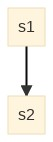
\includegraphics{figure1}
  \caption{eine kleine Menge von Sätzen\label{fig:smallset}}
\end{figure}

Wenn Theorien und Überzeugungen im Modell von \citeauthor{beisbart_making_2015} angepasst werden müssen, so funktioniert dies nach einem einfach beschriebenen Rezept:

\begin{quote}
    [...] the agent newly adopts an epistemic state $(C_i, T_{i+1})$ such that the theory $T_{i+1}$ scores best in terms of the achievement function $Z$ given $C_i$. \autocite[S.~11]{beisbart_making_2015}
\end{quote}

Die Theorie, welche den höchsten Wert der \textit{Achievement-Funktion} $Z$ hat, wird als neue Theorie übernommen. Aber wie findet man heraus, welche Theorie das ist? Man überprüft jede mögliche, konsistent Theorie. Die Menge dieser Theorien ist vor allem aus der Menge an Sätzen im Thema bestimmt - zu einem kleineren Teil aus den Inferenzbeziehungen zwischen den Sätzen. Je mehr Sätze, umso mehr mögliche Theorien. Das Problem ist, dass die Zahl der möglichen Theorien exponentiell zur Zahl der Sätze im Thema wächst. Jeder zusätzliche Satz in einem Thema verdreifacht die Anzahl der möglichen Theorien. Ausserdem muss beachtet werden, dass ein Satz oder seine Negation Prinzip einer Theorie sein kann oder er ist nicht dabei. Das sind pro Satz 3 mögliche Werte. Aus den Überlegungen ist die Zahl der zu überprüfenden Theorien pro Anpassungsschritt $\lvert T \rvert = 3^n$, wobei $n$ die Zahl der Sätze im Thema ist.

Bei den Überzeugungen sieht es leider nicht besser aus: Auch hier werden analog zu den Theorien alle möglichen Überzeugungen überprüft. Erschwerend kommt hinzu, dass die Menge der Überzeugungen nicht durch Inkonsistenzen aus Inferenzbeziehungen eingeschränkt werden. Weil die Überzeugungen nur \textit{minimal konsistent} sein müssen.

Für eine sehr kleine Menge von Sätzen gelingt eine übersichtliche Darstellung noch. Bei Abbildung \ref{fig:smallset} ist eine sehr kleine Menge von Sätzen abgebildet. Wenn nun \textit{s2} die einzige Überzeugung ist und man dazu die passende Theorie suchen möchte, so würden folgende Kombinationen überprüft: $\{\{\}, s1, s2, \neg s1, \neg s2, \{s1,s2\}, \{s1,\neg s2\}, \{\neg s1, s2 \}, \{\neg s1, \neg s2 \} \}$. In dieser einfachen Struktur können keine Mengen ausgeschlossen werden. Alle 9 Elemente müssten überprüft werden. Wenn nun ein einziges weiteres Element \textit{s3} hinzukäme, müssten 27 Mengen überprüft werden.: Das heisst, der Arbeitsaufwand wächst exponentiell zur Anzahl an Sätzen im System. Dies macht diese Methode unrealistisch in der Benutzung. Ausserdem ist es auffällig, wie schnell und einfach die Anpassung intuitiv gemacht werden kann. Für eine Person ist es auf einen Blick zu erkennen, dass s1 das einzige Prinzip ist, welches infrage kommt. Deshalb muss ein neuer Ansatz entwickelt werden.


\section{Der piecemeal Ansatz}
\begin{quote}
    A rule is amended if it yields an inference we are unwilling to accept; an inference is rejected if it violates a rule we are unwililng to amend. \autocite[S.~64]{goodman_fact_1983}
\end{quote}

%%%%delete me 
\textit{Hier kommt eine beschreibung des Piecemeal Ansatzen in der Literator}
%%%

\subsection{Einzelne Elemente hinzufügen oder entfernen}
Wie \cite[S.25]{beisbart_making_2015} schon feststellten, scheint die einfachste Lösung zu sein, einzelne Commitments oder Prinzipien zu ändern und zumindest \citeauthor{goodman_fact_1983} spricht sich klar für einen piecemeal-Ansatz aus. Der erste Ansatz dreht sich um die Idee, von den bestehenden Überzeugungen bzw. der bestehenden Theorie auszugehen anstatt agnostisch davon auszugehen, dass sich alle möglichen Theorien gleich gut eignen. Man ändert die bestehende Theorie bzw. die bestehenden Commitments um ein einzelnes Element ab und sieht, ob diese abgeänderte Theorie bzw. die abgeänderten Überzeugungen besser zu ihrem Gegenstück passen.

\paragraph{Anpassung der Theorie}
Ausgehend von einer Menge von Überzeugungen $C_i$ wird eine Theorie $T_i$ wie folgt angepasst: 
\begin{enumerate}
    \item \label{1} Alle Sätze (auch die Negationen) des Themas $S$ werden einzeln zu der Menge von Prinzipien in $T_i$ hinzugefügt, falls sie noch nicht enthalten sind und die resultierende Theorie konsistent ist. Falls sie aber enthalten sind, wird die Negation des Satzes hinzugefügt. Die Menge der daraus entstandenen Theorien heisst $T_i^*$.
    \item \label{2}Die Mengen, die entstehen, wenn man einzelne Prinzipien aus $T_i$ entfernt, werden zu $T_i^*$ hinzugefügt.
    %\item Die Mengen, die entstehen, wenn man einzelne Prinzipien in $T_i$ negiert, %werden zu $T_i^*$ hinzugefügt.
    \item \label{3}Die Elemente der Menge der Theorien $T_i^*$ wird mittels Achievement-Funktion $Z$ überprüft.
    \item \label{4}Die Theorie, welche den höchsten Wert bei $Z$ erreicht, wird zu $T_{i+1}$ erklärt, falls ihr $Z$-Wert auch grösser ist als jener von $T_1$ - Ansonsten wird $T_1$ zu $T_{i+1}$.
\end{enumerate}

\paragraph{Anpassung der Überzeugungen}
Ausgehend von einer Theorie $T_i$ wird die Menge der Überzeugungen $C_i$ wie folgt angepasst:
\begin{enumerate}
    \item \label{c1} Alle Sätze des Themas $S$ werden einzeln zu der Menge von Überzeugungen in $C_i$ hinzugefügt, falls sie noch nicht enthalten sind. Falls sie aber enthalten sind, wird die Negation des Satzes hinzugefügt. Die Menge der daraus entstandenen Mengen von Überzeugungen heisst $C_i^*$.
    \item \label{c2} Die Mengen, die entstehen, wenn man einzelne Überzeugungen aus $C_i$ entfernt, werden zu $C_i^*$ hinzugefügt.
    \item \label{c3} Die Elemente der Menge der Überzeugungen $C_i^*$ wird mittels Achievement-Funktion $Z$ überprüft.
    \item \label{c4}Die Menge von Überzeugungen, welche den höchsten Wert bei $Z$ erreicht, wird zu $C_{i+1}$ erklärt, falls ihr $Z$-Wert auch grösser ist als jener von $C_1$ - Ansonsten wird $C_1$ zu $C_{i+1}$
\end{enumerate}

\paragraph{Beispiel}
\begin{figure}[h]
  \centering
  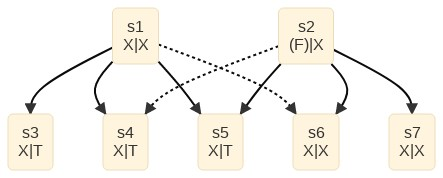
\includegraphics[width=\textwidth]{classical_initial1}
  \caption{Die klassische Struktur im initialen Zustand A\label{fig:classset-initial1}}
\end{figure}

 Als Beispiel für den Ablauf kann die klassische Struktur \ref{fig:classset-initial1} im initialen Zustand mit $C_0 = \{s3, s4, s5\}$ zur Hand genommen werden. Die erste Anpassung der Theorie überprüft nun einfach alle einzelnen Sätze $\{s1,...,s7, \neg s1, ..., \neg s7\}$. Derjenige welche alleine den höchsten Wert von $Z$ erreicht, wird zum einzigen Prinzip. Dies ist $s1$, weil er alle Überzeugungen rechtfertigt und damit wird $\{s1\}$ zu $T_0$.
 
 Die Überzeugungen müssen als Nächstes angepasst werden. Dazu überprüfen wir die Menge von Mengen welche $C_0$ und einen weiteren Satz enthalten. Im Schritt \ref{c1} werden ausserdem alle Mengen erstellt, die entstehen, wenn man einzelne Sätze in $C_0$ negiert, zum Beispiel $\{\lnot s3, s4, s5\}$. Ausserdem überprüfen wir entsprechend Schritt \ref{c2} die Mengen, welche entstehen, wenn man einen einzelnen Satz aus $C_0$ entfernt. Die Überzeugungen werden dahingehend verändert, dass entweder $\neg s6$ oder $\neg s2$ hinzugefügt werden, weil dadurch der Parameter \textit{Account} verbessert wird. Dieser wird bei beiden Änderungen im selben Mass verändert, das heisst, es muss eine Entscheidung getroffen werden. Zur Einfachheit des Beispiels gehe ich davon aus, dass zufällig eine die Möglichkeit gewählt wird, $neg s2$ zu den Überzeugungen hinzuzufügen. Ich komme allerdings im Abschnitt \ref{branching} auf die Möglichkeit des \textit{Branching} zu sprechen. $C_1 = \{s3, s4, s5, \neg s2\}$
 
 Bei der zweiten Anpassung der Theorie müssen nun Theorien geprüft werden, welche $s1$ und einen weiteren Satz enthalten und $\{\neg s1\}$. Hierbei kann $\{s1,s2\}$ und $\{s1,s6\}$ ausgeschlossen werden, weil die Theorien inkonsistent ist. Auch die Theorien aus $s1$ und einem negierten Satz müssen überprüft werden: $\{\{s1,\neg s2\}, \{s1,\neg s7\}, \{s1,\neg s6\}\}$ .Ausserdem muss die leere Theorie überprüft werden - denn sie resultiert aus Schritt \ref{2}. Das Resultat ist, dass keine der überprüften Theorien besser ist als $T_1$. Somit wird $T_1$ auch zu $T_2$ übernommen.
 
 Es folgt eine weitere Anpassung der Überzeugungen. Da sich die Theorie nicht verändert hat, liegt auf der Hand, dass das Hinzufügen von $\neg s6$ zu $C_1$ die beste Alternative ist. Somit sieht $C_2$ nun wie folgt aus: $C_2 = \{s3, s4, s5, \neg s2, \neg s6\}$
 
 Weil $T_2$ mit $T_1$ identisch ist, müssen auch dieselben Theorien überprüft werden. Das Ergebnis wird sich nicht verändern und $T_3$ wird mit $T_2$ gleichgesetzt.
 
 Es folgt eine letzte Überprüfung der Überzeugungen. Nach dem beschriebenen Rezept wird diese wieder durchgeführt, mit dem Ergebnis, dass es keine Verbesserung gibt und $C_3$ mit $C_4$ gleichgesetzt wird. Damit endet der Prozess mit dem Ergebnis eines Reflective Equilibriums.
 
 Während des Prozesses mussten in der ersten Änderung 14 Theorien und in der zweiten und dritten Änderung neun Theorien überprüft und verglichen werden.  Im Vergleich zum traditionellen Ansatz, bei dem in jedem Schritt $3^7$ Theorien (ohne Berücksichtigung der inkonsistenten Theorien) überprüft und verglichen werden. In der Anpassung der Überzeugungen müssen bei jedem Schritt immer $2t + 1$ Überzeugungen überprüft werden. Wobei $t$ der Anzahl von Sätzen im Topic entspricht. Für das Beispiel heisst das $15$ Überprüfungen pro Anpassung. Beim traditionellen Ansatz müssen bei jedem Schritt wieder $3^7$ Überzeugungen überprüft werden. Wichtig für die Frage, ob der traditionelle Ansatz wirklich weniger effizient ist, ist neben der Anzahl zu überprüfenden Mengen pro Schritt auch die Anzahl der Schritte. Diese wäre für unser Beispiel für das traditionelle Modell 4 Schritte (2 für die Überzeugungen und 2 für die Theorien), für den neuen Ansatz sind es 7 Schritte. Die Anzahl Schritte ist 1.75 Mal höher, aber die Anzahl von Rechenschritten pro Schritt ist $145.8$ Mal höher. Wenn sich bei weiteren Kompositionen ähnliche Werte ergeben, ist die neue Methode der traditionellen vorzuziehen. Ausserdem gilt es zu überprüfen, ob die Methode globale Optima erreicht.
 % Run the numbers again...

\subsection{Analyse der Inferenzbeziehungen}
Eine weitere Idee, einen piecemeal-Ansatz umzusetzen, ist die Analyse der gegebenen Inferenzbeziehungen. Aufgrund der Inferenzbeziehungen zwischen Sätzen, kann klug entschieden werden, welche Sätze sich eher als Theorien lohnen. Auch für die Anpassung der Überzeugungen kann es hilfreich sein, zu analysieren, welche Inferenzbeziehungen die zuletzt hinzugefügten Prinzipien haben.

\paragraph{Anpassung der Theorie}
Ausgehend von einer Menge von Überzeugungen $C_i$ wird eine Theorie $T_i$ wie folgt angepasst. Hierbei entspricht $z$ der Anzahl Durchläufe und $c_a$ der aktuell ausgewählten Überzeugung. 
\begin{enumerate}
    \item \label{i1} Die erste Überzeugung aus $C_i$ wird ausgewählt: $c_a = c_0$ (Index 0)
    \item \label{i2} Falls die Menge $S_z$ leer ist: Für die ausgewählte Überzeugung $c_a$ werden alle Prinzipien gesucht, welche die ausgewählte Überzeugung zum Inhalt haben. Jedes gefundene Prinzip eröffnet eine neue Menge und diese Mengen werden $S_z$ hinzugefügt. Falls $S_z$ nicht leer ist: Jedes für $c_a$ gefundene Prinzip wird zu den Mengen in $S_z$ hinzugefügt, falls die entstehende Menge konsistent ist und das Prinzip nicht schon enthalten ist.
    \item \label{i3} Falls $c_x$ noch nicht das letzte Element aus $C_i$ ist, wird die nächste Überzeugung aus $C_i$ wird ausgewählt und zu Schritt \ref{i2} gesprungen.
    \item \label{i4} Falls $z < \lvert C_i \rvert$: Die Reihenfolge der Überzeugungen in $C_i$ wird geändert. Dabei wird die erste Überzeugung zur letzten. $z$ wird um eins inkrementiert: $z = z + 1$ und zu Schritt \ref{i1} gesprungen. %Achtung: Vielleicht müssen alle Permutationen von C_i geprüft werden? Es macht definitiv einen unterschied... die Frage ist, ob es auch schlechter funktioniert...
    \item \label{i5} In den Mengen $S_\alpha$ werden die Mengen, welche die gleichen Elemente enthalten zu einer reduziert. Alle $S_\alpha$ Mengen werden mittels Achievement-Funktion $Z$ überprüft.
    \item \label{i6}Die Theorie, welche den höchsten Wert bei $Z$ erreicht, wird die Theorie $T_i$ ersetzen und zu $T_{i+1}$ erklärt, ausser ihr Wert ist kleiner als der Wert von $T_i$. In diesem Fall wird $T_i$ zu $T_{i+1}$ erklärt.
    %Danach werden zu allen Mengen in den $S_\alpha$ Mengen die Überzeugungen hinzugefügt, die nicht aus anderen Sätzen folgen.% Müssen alleinstehende Überzeugungen überhaupt berücksichtigt werden?
\end{enumerate}

\paragraph{Anpassung der Überzeugungen}
Ausgehend von einer Theorie $T_i$ werden für $C_i+1$ die Prinzipien und der Inhalt von $T_i$ übernommen.
Durch diesen Schritt wird immer voller \textit{Account} garantiert, dafür wird $C_0$ aber vernachlässigt und somit \textit{Faithfulness} gefährdet. Es muss durch Experimente gezeigt werden, ob dieser Ansatz zu gleich guten Ergebnissen führt wie der traditionelle Ansatz.

\paragraph{Beispiel}
Beispielhaft kann auch hier wieder die Struktur, welche auf Abbildung \ref{fig:classset-initial1} illustriert ist, dienen. Im ersten Schritt wählen wir $s3$ und finden $s1$ als mögliches Prinzip für $s3$ im zweiten Schritt. Da $S_0$ noch leer ist, fügen wir $s1$ hinzu. Dann suchen wir ein Prinzip für $s4$, wobei wir wieder auf $s1$ stossen und dieses nicht ein zweites Mal zu $S_0$ hinzufügen. Danach folgt unsere nächste und letzte Überzeugung $s5$. Für $s5$ finden wir nun zwei mögliche Prinzipien: $s1$ und $s2$. Nun ergäben sich zwei Mengen in $S_0$: $\{s1\}$ und $\{s1, s2\}$. Da $\{s1, s2\}$ aber inkonsistent ist, wird sie weggelassen. Als Nächstes starten wir den Prozess erneut, diesmal fangen wir aber mit $s4$ als erster Überzeugung an, für die wir Prinzipien suchen. Der Prozess verläuft analog zum ersten Durchgang, und am Ende haben wir eine Menge $S_1 = \{s1\}$. Für den dritten und letzten Durchgang mit $s5$ als Startüberzeugung ergibt sich aber ein anderes Bild: Zu $S_2$ werden die beiden Prinzipien $s1$ und $s2$ als einzelne Elemente hinzugefügt. Bei der Suche nach einem Prinzip für $s4$ und analog für $s3$ wird jeweils $s1$ gefunden. Zur ersten Menge in $S_2$ wird $s1$ nicht hinzugefügt, weil es schon darin ist, zur zweiten Menge nicht, weil die resultierende Menge $\{s1,s2\}$ inkonsistent wäre. Somit ist $S_1 = \{{s1}, {s2}\}$. Die Mengen in $S_0$, $S_1$ und $S_3$ werden nun zusammengeführt, wobei die Doppelungen wieder gestrichen werden können. Somit ergeben sich folgende Kandidaten, für die ihr $Z$-Wert verglichen werden muss: $\{{s1}, {s2}\}$.

\newpage
\printbibliography

\end{document}


%%%%%%%%%%%%%%%%%%%%%%%%


\begin{enumerate}
    \item How can logic be defined in a general way, so that different rival theories can be understood as \textit{logical} theories?
\end{enumerate}

\begin{quote}
    An argument is logically valid just when conditional [sic.], with the conjunction of the premises as antecendent and the conclusion as consequent, is logically true. We can readily slip from one notion to the other[...] \cite[p.~13]{beallrestall}
\end{quote}

\subsection{Debating on logic}\label{sec:debating}
\footnote{An extensive discussion of trivialism and why it is an irrational view can be found in chapter 3 of \citeA{priest2}.}

 \fullciteauthor{beallrestall}

(see section \ref{principle:GGTP}, page \pageref{principle:GGTP})

\begin{center}
\begin{tabular}{c p{9cm}}
P1 & If I am king of France, I'm not king of France.\\\hline
C & If I am king of France, God exists. 
\end{tabular}
\end{center}

\paragraph{Systematicity} To define the consequence relation by specifying it for each argument separately would be a very unsystematic procedure. \textbf{Systematicity}, like the one brought forward by \citeauthor{resnik0} or \citeauthor{peregrinsvoboda}. They have, as I will argue, a problematic understanding of the purpose of an RE-process.